\documentclass{article}
\usepackage[letterpaper, margin=0.1in]{geometry}
\usepackage{multicol}
\usepackage{graphicx}
\usepackage{amsmath}
\usepackage{array}
\usepackage{xcolor,colortbl}


\begin{document}
\LARGE
\section{Trigonometery Table}
\centering
\renewcommand{\arraystretch}{2}
\newcommand\Bstrut{\rule[-1.3em]{0pt}{0pt}}  

\begin{tabular}{|c|c|c|c|c|c|c|c|}
    \hline
    Angle $(^\circ)$ & $0^\circ$ & $30^\circ$ & $45^\circ$ & $60^\circ$ & $90^\circ$ & $180^\circ$ & $270^\circ$\Bstrut\\
    \hline
    Angle $(Radians)$ & $0$ & $\dfrac{\pi}{6}$ & $\dfrac{\pi}{4}$ & $\dfrac{\pi}{3}$ & $\dfrac{\pi}{2}$ & $\pi$ & $\dfrac{3\pi}{2}$ \Bstrut\\
    \hline
        $\sin$ & $0$ & 
        $\dfrac{1}{2}$ & 
        $\dfrac{1}{\sqrt{2}}$ & 
        $\dfrac{\sqrt{3}}{2}$ & 
        $1$ & 
        $0$ & 
        $-1$ 
        \Bstrut\\
    \hline
        $\cos$ & $1$ & 
        $\dfrac{\sqrt{3}}{2}$ & 
        $\dfrac{1}{\sqrt{2}}$ & 
        $\dfrac{1}{2}$ & 
        $0$ & 
        $-1$ & 
        $0$ 
        \Bstrut\\
    \hline
        $\tan$ & $0$ & 
        $\dfrac{1}{\sqrt{3}}$ & 
        $1$ & 
        $\sqrt{3}$ & 
        Undefined & 
        $0$ & 
        Undefined 
        \Bstrut\\
    \hline
        $\csc$ & Undefined & 
        $2$ & 
        $\sqrt{2}$ & 
        $\dfrac{2}{\sqrt{3}}$ & 
        $1$ & 
        Undefined & 
        $-1$ 
        \Bstrut\\
    \hline
        $\sec$ & $1$ & 
        $\dfrac{2}{\sqrt{3}}$ & 
        $\sqrt{2}$ & 
        $2$ & 
        Undefined &
        $-1$ &
        Undefined 
        \Bstrut\\
    \hline
        $\csc$ & Undefined & 
        $\sqrt{3}$ & 
        $1$ & 
        $\dfrac{1}{\sqrt{3}}$ & 
        $0$ & 
        Undefined & 
        $0$ 
        \Bstrut\\
    \hline
\end{tabular}
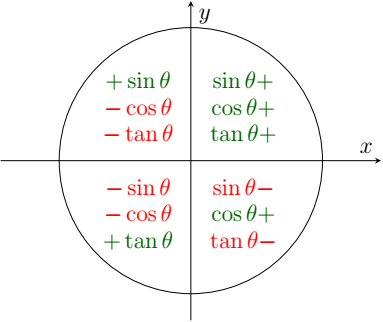
\includegraphics{images/trig-quadrants.png} \\
\end{document}